%\documentclass[iop]{emulateapj}
\documentclass[aps, prl, twocolumn, nofootinbib, groupedaddress, amsfonts, amssymb, amsmath]{revtex4-1}
\usepackage{graphicx}
\usepackage{bm}
\usepackage{natbib}
%\usepackage[colorlinks=True, linkcolor=blue, citecolor=blue]{hyperref}
%\usepackage[all]{hypcap}

\bibliographystyle{apsrev}

\newcommand{\Div}[1]{\ensuremath{\nabla\cdot\left( #1\right)}}
\newcommand{\angles}[1]{\ensuremath{\left\langle #1 \right\rangle}}
\newcommand{\grad}{\ensuremath{\nabla}}
\newcommand{\RB}{Rayleigh-B\'{e}nard }
\newcommand{\stressT}{\ensuremath{\bm{\bar{\bar{\Pi}}}}}
\newcommand{\lilstressT}{\ensuremath{\bm{\bar{\bar{\sigma}}}}}
\newcommand{\nrho}{\ensuremath{n_{\rho}}}
\newcommand{\approptoinn}[2]{\mathrel{\vcenter{
	\offinterlineskip\halign{\hfil$##$\cr
	#1\propto\cr\noalign{\kern2pt}#1\sim\cr\noalign{\kern-2pt}}}}}

\newcommand{\appropto}{\mathpalette\approptoinn\relax}

\newcommand\mnras{{MNRAS}}%
          % Monthly Notices of the RAS

\begin{document}
%%%%% Create nice title and abstract
\author{Evan H. Anders}
\affiliation{Department of Astrophysical \& Planetary Sciences, University of Colorado -- Boulder}
\affiliation{Laboratory for Atmospheric and Space Physics, Boulder, CO}
\author{Benjamin P. Brown}
\affiliation{Department of Astrophysical \& Planetary Sciences, University of Colorado -- Boulder}
\affiliation{Laboratory for Atmospheric and Space Physics, Boulder, CO}
\title{Convective heat transport in stratified atmospheres at low and high Mach number}

\begin{abstract}
Convection in astrophysical systems is stratified and
often occurs at high Rayleigh number (Ra) and low
Mach number (Ma).
Here we study stratified convection in the context of 
plane-parallel, polytropically stratified atmospheres. 
We hold the density stratification ($n_{\rho}$) and Prandtl 
number (Pr) constant while varying the superadiabaticity
and Ra.  We find that Ma is primarily controlled by the
superadiabaticity of the atmosphere.  We also examine
the behavior of the Nusselt number (Nu), 
which quantifies the efficiency of convective heat transport,
and the Reynolds number (Re), which quantifies how turbulent our
solutions are.
%As Ra increases and $\text{Ma} \rightarrow 1$, a scaling 
%of Nu $\propto$ Ra$^{0.45}$ is observed.  
%As Ra increases to a regime where Ma $\geq 1$,
%this scaling gives way to a weaker Nu $\propto$ Ra$^{0.19}$. 
%In the regime of Ma $\ll 1$, a consistent
%Nu $\propto$ Ra$^{0.31}$ is retrieved,  reminiscent of the 
%Nu $\propto$ Ra$^{2/7}$ seen in \RB convection.
\end{abstract}
\maketitle


%%%%% Body of the paper
\section{Introduction}
\refstepcounter{section}
\label{sec:intro}
Convective heat transport is essential
in the cores of high mass stars,
the envelopes of low mass stars, and the atmospheres of terrestrial and 
jovian planets.  These astrophysical systems have density stratifications
ranging from a few density scale heights (e.g. massive star cores)
up to 14 density scale heights in the convective envelopes of low
mass stars such as the Sun.
Atmospheric stratification presumably modifies the fundamental
dynamics and heat transport mechanisms of these atmospheres.
Understanding the fundamental
properties of compressible convection in stratified media is essential
to characterizing systems in astrophysics and planetary sciences.  
Numerical constraints have often restricted studies of compressible
convection to moderately high Mach number (Ma), appropriate to regions near 
the Sun's surface.  Few fundamental properties of
low Ma convection, which occurs in the deep solar interior, are known.

Early numerical experiments on stratified convection
in two \cite{graham1975, chan&all1982,
hurlburt&all1984, cattaneo&all1990} and three 
\cite{cattaneo&all1991, brummell&all1996} dimensions
revealed a number of basic properties in the moderate-to-high 
Ma regime. In the widely-studied \RB (hereafter RB) problem, 
upflows and downflows are symmetrical and
the conductive flux approaches zero in the convective interior.
These two hallmark characteristics of RB convection change
significantly when stratification is included.  Stratified convection 
exhibits narrow downflow lanes and broad upflow regions.
Furthermore, the \emph{entropy} gradient is negated by convection 
rather than the temperature gradient, and
a significant conductive flux can exist in the presence of
efficient convection.

In RB convection, there exist two primary control parameters: 
the Rayleigh number (Ra, the ratio of
buoyant driving to diffusive damping) and the Prandtl number 
(Pr, the ratio of viscous to thermal
diffusivity).  These numbers coupled with the aspect ratio of 
the physical domain and the boundary conditions
determine the dynamics of the convection.  In stratified atmospheres, 
in addition to specifying the equation of state and
fundamental properties of the gas, the two control parameters of 
RB convection are joined by the degree of
stratification across the domain and the characteristic 
Ma of the convective flows.  
Polytropically stratified atmospheres, such as those used in 
early studies \cite{graham1975, chan&all1982, hurlburt&all1984, 
cattaneo&all1990, cattaneo&all1991, brummell&all1996}, are an ideal extension of
RB convection into the stratified realm because the two additional 
control parameters are directly linked to
basic properties of the atmosphere.  The density stratification is 
set by the number of density scale heights (\nrho)
the atmosphere spans, and Ma is controlled 
by the superadiabatic excess ($\epsilon$),
the deviation of the polytropic index from the adiabatic polytropic 
index \cite{graham1975}.

In this letter we study the behavior of convective heat transport, 
quantified by the Nusselt number (Nu), in plane-parallel, 
two-dimensional, polytropically stratified atmospheres.  
We vary $\epsilon$ and Ra while holding $\nrho$, Pr, and the aspect ratio
constant.  We describe experimental methods in section 
\ref{sec:experiment}, including the construction of atmospheres, equations, and numerical methods.  
Results are described in section \ref{sec:results} and their implications are discussed
in section \ref{sec:discussion}.

\section{Experiment} 
\refstepcounter{section}
\label{sec:experiment}
We exmine the simplest stratified extension of RB by studying a
fluid composed of monatomic ideal gas particles with an adiabatic 
index of $\gamma = 5/3$ and whose equation of state is $P = R\rho T$. 
This is consistent with the approach used in earlier work.
The initial atmosphere is a plane-parallel polytrope in which 
the gravitational acceleration and conductive flux, 
$\bm{F}_{\text{cond,0}} = -\kappa \partial_z T_0$, do not vary with depth. To
achieve the latter condition, both $\kappa$ and $\partial_z T_0$ are constant.
Under these assumptions, satisfying hydrostatic 
equilibrium produces a stratification of
\begin{equation}
\begin{split}
\rho_0(z) &= \rho_{t}(z_0 - z)^m, \\
T_0(z)    &= T_{t}(z_0 - z),
\label{eqn:polytrope}
\end{split}
\end{equation}
where $m = m_{\text{ad}} - \epsilon$ is the polytropic index.
The adiabatic polytropic index is $m_{\text{ad}} \equiv (\gamma-1)^{-1}$, and
the superadiabatic excess is $\epsilon$ which sets the scale 
of the entropy gradient ($\partial_z S_0 \propto -\epsilon$).
A significant advance of this work is the ability to study large 
and small values of $\epsilon$, as will be discussed.
Thermodynamic variables are nondimensionalized at the 
top of the atmosphere as  $P_0(L_z) = \rho_0(L_z) = T_0(L_z) = 1$, 
requiring $z_0 \equiv L_z + 1$ and $R = T_{t} = \rho_{t} = 1$.
By this choice, the non-dimensional length scale is the inverse 
temperature gradient scale and the timescale is the isothermal 
sound crossing time of this unit length.
The height $z$ increases upwards within $[0, L_{z}]$, 
where $L_{z} = e^{n_{\rho}/m} - 1$ is
determined by $n_\rho$ and $\epsilon$.
The characteristic timescale of convective dynamics
is related to the atmospheric buoyancy time, 
$t_{\text{b}} = \sqrt{L_z/g\epsilon}$, with $g = (m+1)$.
Throughout this letter, we use buoyancy time units and 
choose $n_{\rho} = 3$ such that the 
initial density varies by a factor of 20.
All atmospheres studied here have an aspect ratio of 4, 
such that $L_x = 4L_z$.

The atmospheric diffusivities are primarily controlled by
the non-dimensional Rayleigh number,
\begin{equation}
\text{Ra} = \frac{g L_z^3 (\Delta S_0 / c_P)}{\nu\chi},
\end{equation}
where $\Delta S_0 = \epsilon\ln z_0$ is the entropy difference 
between the top and bottom boundaries, 
$c_P = R\gamma(\gamma-1)^{-1}$ is the specific heat 
at constant pressure, $\nu$ is the kinematic viscosity 
(the viscous diffusivity), and $\chi$ is the thermal diffusivity.  
The relationship between the thermal and viscous diffusivities is
set by the Prandtl number, $\text{Pr} = \nu/\chi$.   
The dynamic viscosity, $\mu$, and the thermal conductivity,
$\kappa$, relate to their corresponding diffusivities such that 
$\nu \equiv \mu/\rho$ and $\chi \equiv \kappa/\rho$.  We take
$\mu$ and $\kappa$ to be constant with height.
As a result, $\text{Ra} \propto (\nu\chi)^{-1} \propto
\rho^2$.  The atmospheres studied here with $n_{\rho} = 3$ 
experience an increase in Ra 
by a factor of 400 across the domain.  This formulation leaves Pr
constant throughout the depth of the atmosphere. 
In this letter we impose $\text{Pr} = 1$ and specify Ra at 
the top of the domain ($z = L_z$). 

While holding $n_\rho$ and Pr constant, 
the primary control parameters of convection are $\epsilon$
and Ra.  We decompose our atmosphere into the background 
polytrope ($\ln\rho_{0}, T_{0}$) and the fluctuations
about that background ($\bm{u}, \ln\rho_{1}, T_{1}$),
which can be large.
The scaling of the entropy gradient with $\epsilon$
is reflected in the evolved values of these fluctuations.  For small $\epsilon$,
evolved values scale as
$T_1/T_0 \propto \rho_{1}/\rho_{0} \propto$ Ma$^{2} \propto \epsilon$,
as shown in Fig. \ref{fig:ma_v_eps}.  

\begin{figure}[t]
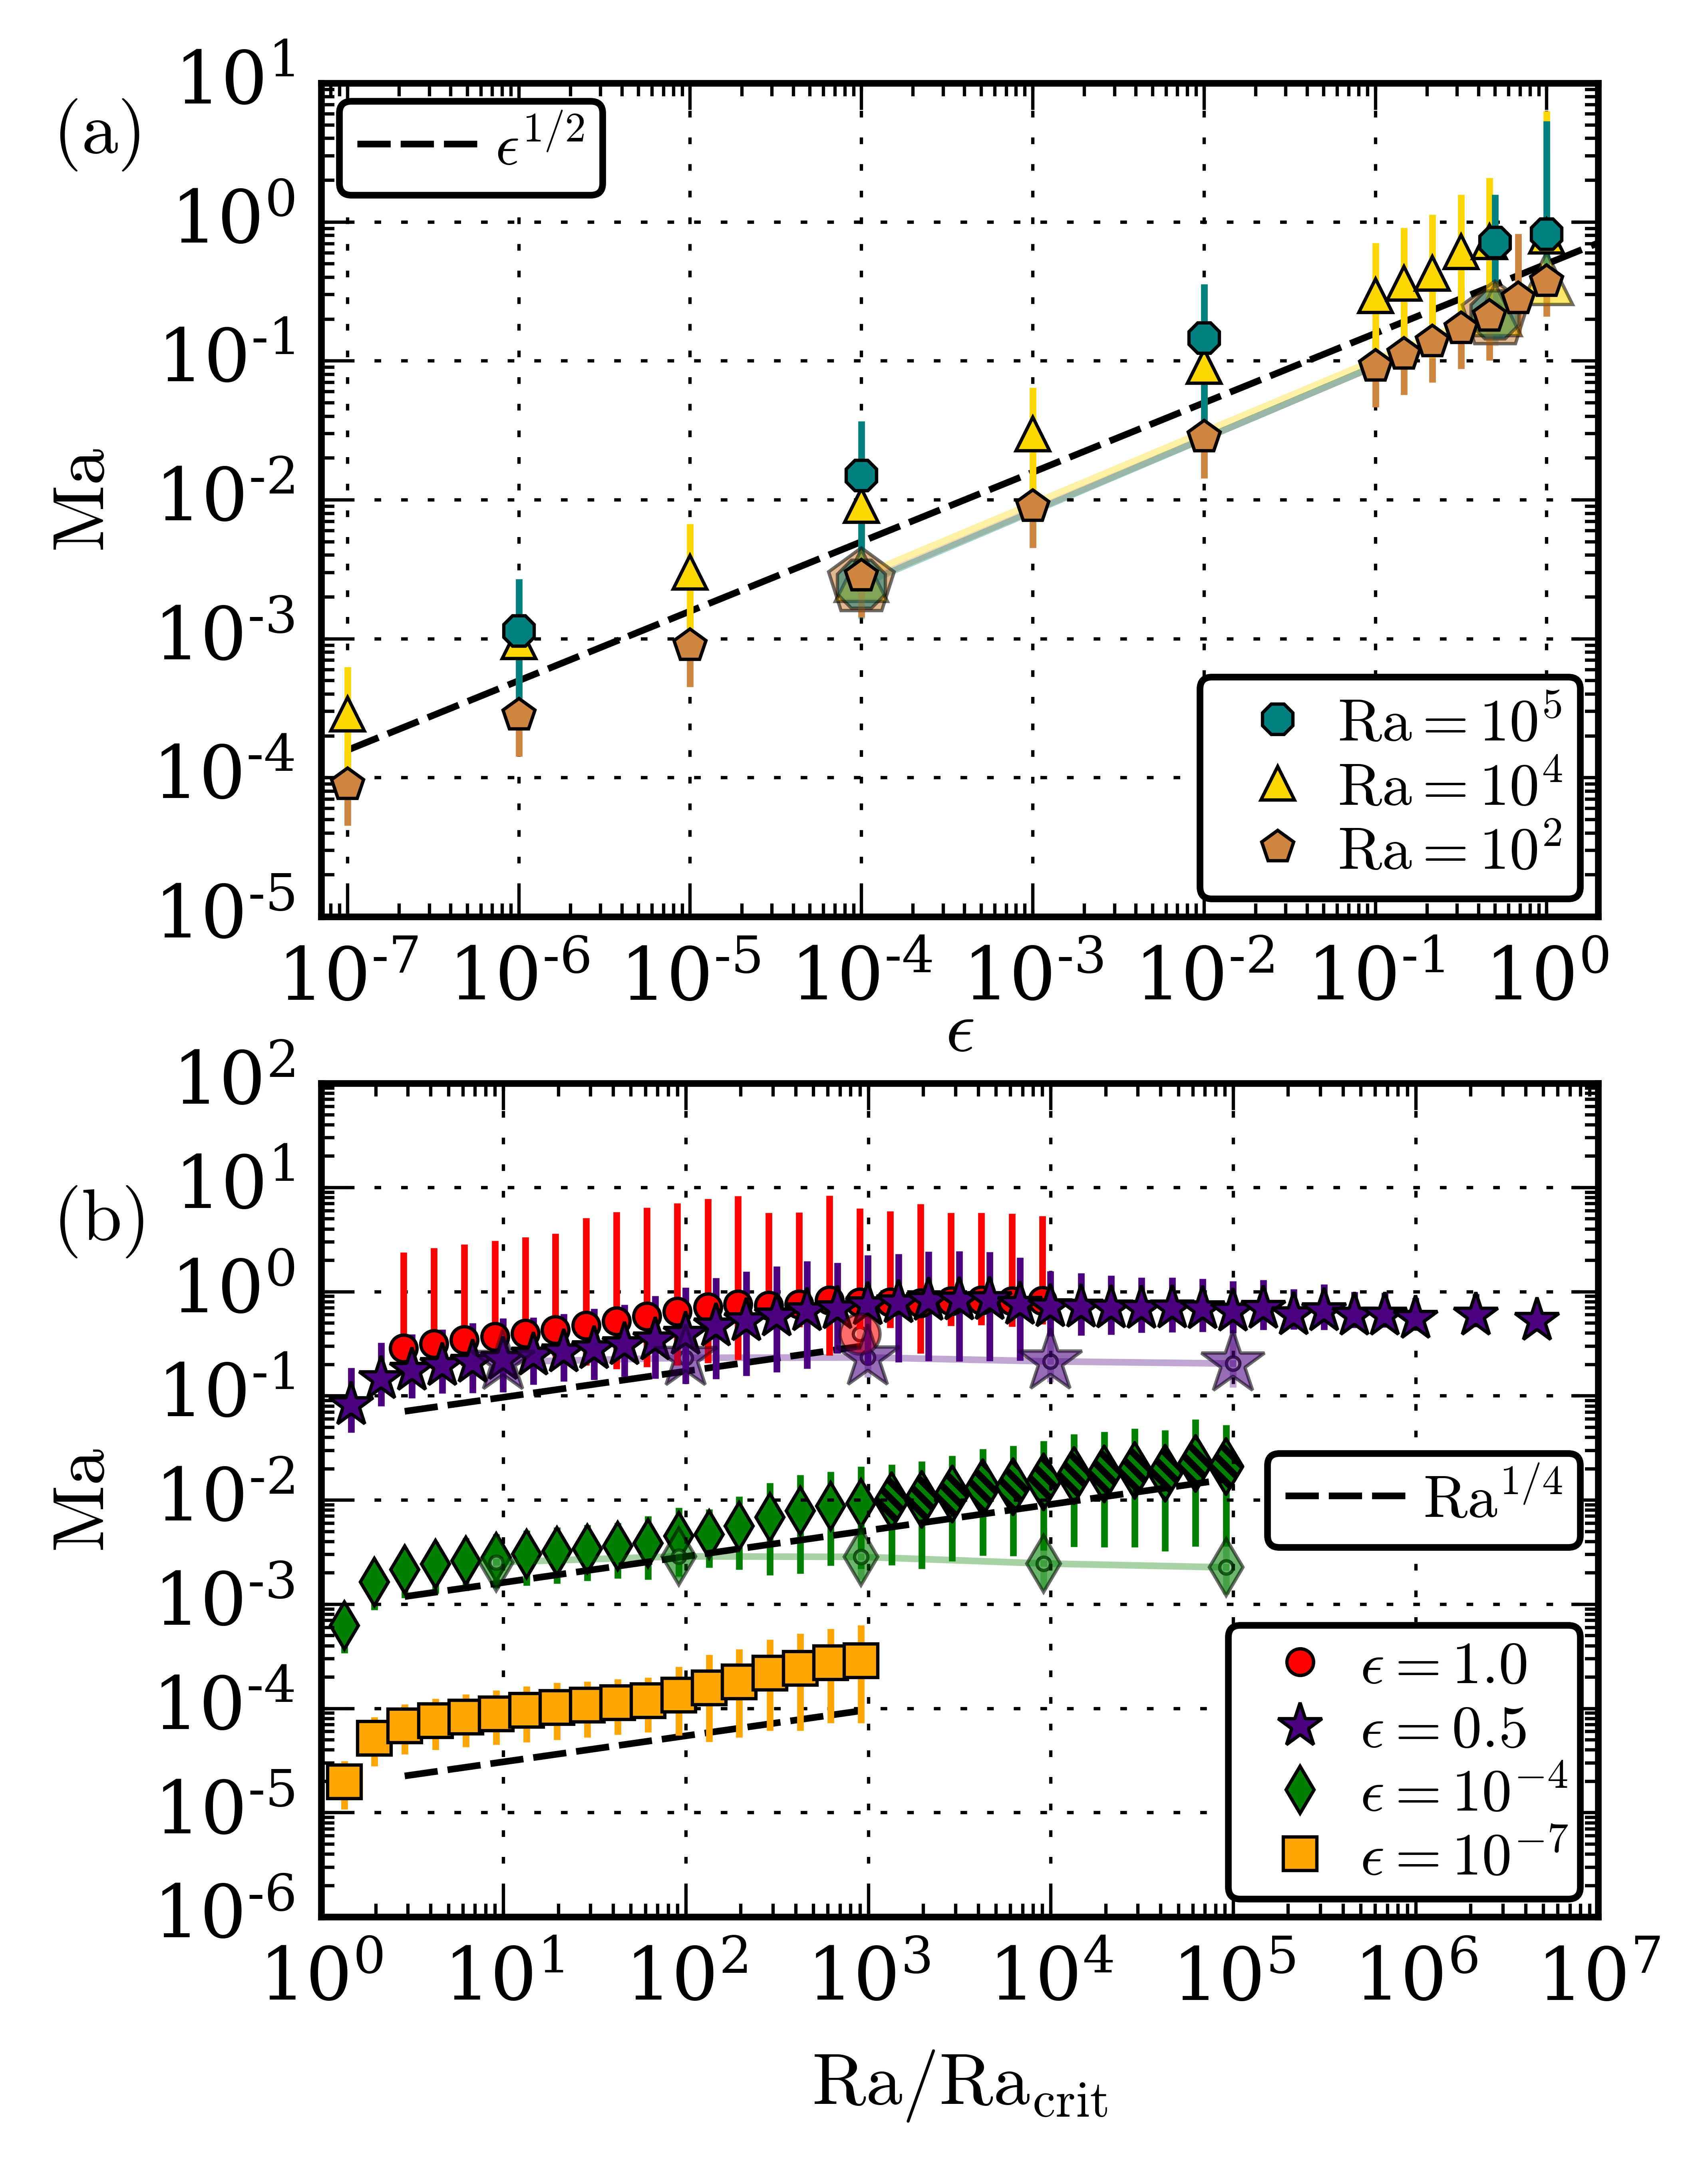
\includegraphics[width=3.4375in]{./figs/ma_v_Ra.png}
\caption{The maximum value of Ma which has been horizontally 
averaged and time averaged for $\geq 100 t_b$, 
beginning roughly $50t_b$ after
the start of simulations.  This time average is long 
enough that the profile is well converged
and error bars are negligible. (a) For $\epsilon \leq 0.1$,
a scaling of $\text{Ma }\propto \{\epsilon^{0.50}, \epsilon^{0.51}\}$ 
at $\text{Ra }= \{10^2, 10^5\}$ exists.
When $\epsilon \rightarrow m_{\text{ad}}$, 
large deviations from this power law are seen.  
(b) At high $\epsilon$, Ma scales as Ra$^{0.28}$ 
until it reaches the supersonic regime, at which point it
follows a power law of Ra$^{-0.10}$.  At low $\epsilon$, 
consistent power laws are achieved throughout all
values of Ra studied, where 
$\text{Ma }\propto \{\text{Ra}^{0.26},\,\text{Ra}^{0.22}\}$
for $\epsilon = \{10^{-4}, 10^{-7}\}$. 
\label{fig:ma_v_eps} }
\end{figure}

We evolve the Fully Compressible Navier-Stokes equations,
\begin{align}
&\begin{aligned}
&\frac{\partial \ln\rho}{\partial t} + \grad\cdot\bm{u} 
    = -\bm{u}\cdot\grad\ln\rho,
	\label{eqn:continuity_eqn}
\end{aligned}\\
&\begin{aligned}
\frac{\partial\bm{u}}{\partial t} + \grad T - 
&\nu\grad\cdot\lilstressT - \lilstressT\cdot\grad\nu = \\
&-\bm{u}\cdot\grad\bm{u} - T\grad\ln\rho + \bm{g} + 
\nu\lilstressT\cdot\grad\ln\rho,
\label{eqn:momentum_eqn}
\end{aligned}\\
&\begin{aligned}
\frac{\partial T}{\partial t} -\frac{1}{c_V}\left(\right.\chi&\left.
    \grad^2 T + \grad T\cdot\grad\chi\right) = \\
	&-\bm{u}\cdot\grad T - (\gamma-1)T\grad\cdot{\bm{u}} \\
	&+ \frac{1}{c_V}\left(\chi\grad T \cdot\grad\ln\rho +
	\nu\left[\lilstressT\cdot\nabla\right]\cdot\bm{u}\right), 
	\label{eqn:energy_eqn}
\end{aligned}
\end{align}
with the viscous stress tensor given by
\begin{equation}
\sigma_{ij} \equiv \left(\frac{\partial u_i}{\partial x_j} + 
\frac{\partial u_j}{\partial x_i} - \frac{2}{3}\delta_{ij}\grad\cdot\bm{u}\right).
	\label{eqn:stress_tensor}
\end{equation}
Taking an inner product of
(\ref{eqn:momentum_eqn}) with $\bm{u}$ and adding it to 
(\ref{eqn:energy_eqn}) reveals the full energy equation,
\begin{equation}
\frac{\partial}{\partial t}\left(\rho\left[\frac{|\bm{u}|^2}{2} + c_V T + \phi\right]\right) +
\Div{\bm{F}_{\text{conv}} + \bm{F}_{\text{cond}}} = 0,
	\label{eqn:energy_eqn_full}
\end{equation}
where
$
\bm{F}_{\text{conv}} \equiv \bm{F}_{\text{enth}} + \bm{F}_{\text{KE}} + \bm{F}_{\text{PE}} + \bm{F}_{\text{visc}}
$
is the convective flux and $\bm{F}_{\text{cond}} = -\kappa \grad T$
is the conductive flux.
The individual contributions to $\bm{F}_{\text{conv}}$ are the enthalpy flux, 
$\bm{F}_{\text{enth}} \equiv \rho\bm{u}(c_V T + P/\rho)$;
the kinetic energy flux, 
$\bm{F}_{\text{KE}} \equiv \rho|\bm{u}|^2\bm{u}/2$;
the potential energy flux,
$\bm{F}_{\text{PE}} \equiv \rho\bm{u}\phi$ (with $\phi \equiv -gz$);
and the viscous flux, 
$\bm{F}_{\text{visc}} \equiv -\rho\nu\bm{u}\cdot\lilstressT$, and each 
must be considered. 
Understanding how these fluxes interact  
is crucial in characterizing convective heat transport.

The atmosphere is contained between two 
impenetrable, stress free, fixed temperature boundaries at
the top and bottom of the domain such that 
$w = \partial_z u = T_1 = 0$ at $z = \{0, L_z\}$. The domain
is horizontally periodic. We utilize the 
Dedalus\footnote{http://dedalus-project.org/} \cite{burns&all2016} pseudospectral framework 
 to time-evolve  
(\ref{eqn:continuity_eqn})-(\ref{eqn:energy_eqn}) 
using an implicit-explicit, third-order, four-step 
Runge-Kutta timestepping scheme RK443 \cite{ascher&all1997}.  
Variables are time-evolved on a dealiased Chebyshev (vertical)
and Fourier (horizontal) domain in which the
physical grid dimensions are 3/2 the size of the coefficient grid.  
Physical grid sizes range from
96x384 grid points at the lowest values of 
Ra to 1152x4608 grid points at Ra $\geq 10^{7}$. 
By using IMEX timestepping, we implicitly step the 
stiff linear acoustic wave contribution and are able to
efficiently study flows at moderate ($\approx 1$) and very low ($\approx 10^{-4}$)
Ma (Fig. \ref{fig:ma_v_eps}b).  Our equations take the form
of the FC equations in \cite{lecoanet&all2014}, extended to include variable
$\nu$ and $\chi$, and we follow the approach there; 
this IMEX approach has been successfully 
tested against a nonlinear benchmark  of the compressible 
Kelvin-Helmholtz instability \cite{Lecoanet_et_al_2016_KH}.

\section{Results}
\refstepcounter{section}
\label{sec:results}

The efficiency of convection is quantified by the Nusselt number.  
Nu is well-defined in RB convection
as the total flux normalized by the steady-state conductive flux 
\cite{johnston&doering2009, otero&all2002}.
In stratified convection Nu is more difficult to define, and we use
a modified version of a traditional stratified Nusselt number \cite{graham1975,hurlburt&all1984},
\begin{equation}
\text{Nu} \equiv \frac{\langle F_{\text{conv, z}} + F_{\text{cond, z}} - F_{\text{A}}\rangle}
{\langle F_{\text{cond, z}} - F_{\text{A}}\rangle} 
= 1 + \frac{\langle F_{\text{conv, z}}\rangle}{\langle F_{\text{cond, z}} - F_{\text{A}} \rangle}
\label{eqn:nusselt}
\end{equation}
where $F_{\text{conv, z}}$ and $F_{\text{cond, z}}$ are the 
z-components of $\bm{F}_{\text{conv}}$ and $\bm{F}_{\text{cond}}$,
respectively and $\langle \rangle$ implies a volume average.  
$F_{\text{A}} \equiv -\langle\kappa\rangle \partial_z T_{\text{ad}}$ 
is the adiabatic conductive flux and
$\partial_z T_{\text{ad}} \equiv - g / c_{P}$ 
for an ideal gas in hydrostatic equilibrium.  Here we specify
$\langle \kappa \rangle = \langle (\rho_{1}/\rho_{0})\kappa_0 \rangle$.
At large values of $\epsilon$, $\kappa$ evolves significantly as the
density profile evolves.  At low $\epsilon$, $\langle\kappa\rangle \approx \kappa_0$.
In the Boussinesq approximation, under which $\grad S = 0$ only when 
$\grad T = 0$, this definition reduces the the traditional definition
of the Nusselt number \cite{otero&all2002, johnston&doering2009}.

The Reynolds number and Peclet number,
\begin{equation}
\text{Re} = \frac{|\bm{u}| L_z}{\nu};\,\,\,\,\text{Pe} = \text{Pr}\,\text{Re},
\end{equation}
quantify the importance of advection to diffusion in the evolved
convective state.  Our choice of $\{\nu,\chi\}\propto \rho_0^{-1}$ drastically changes
the value of Re between the top and bottom of the atmosphere.  We report values of
Re at the midplane ($z=L_z/2$) of the atmosphere.

\begin{figure}[b]
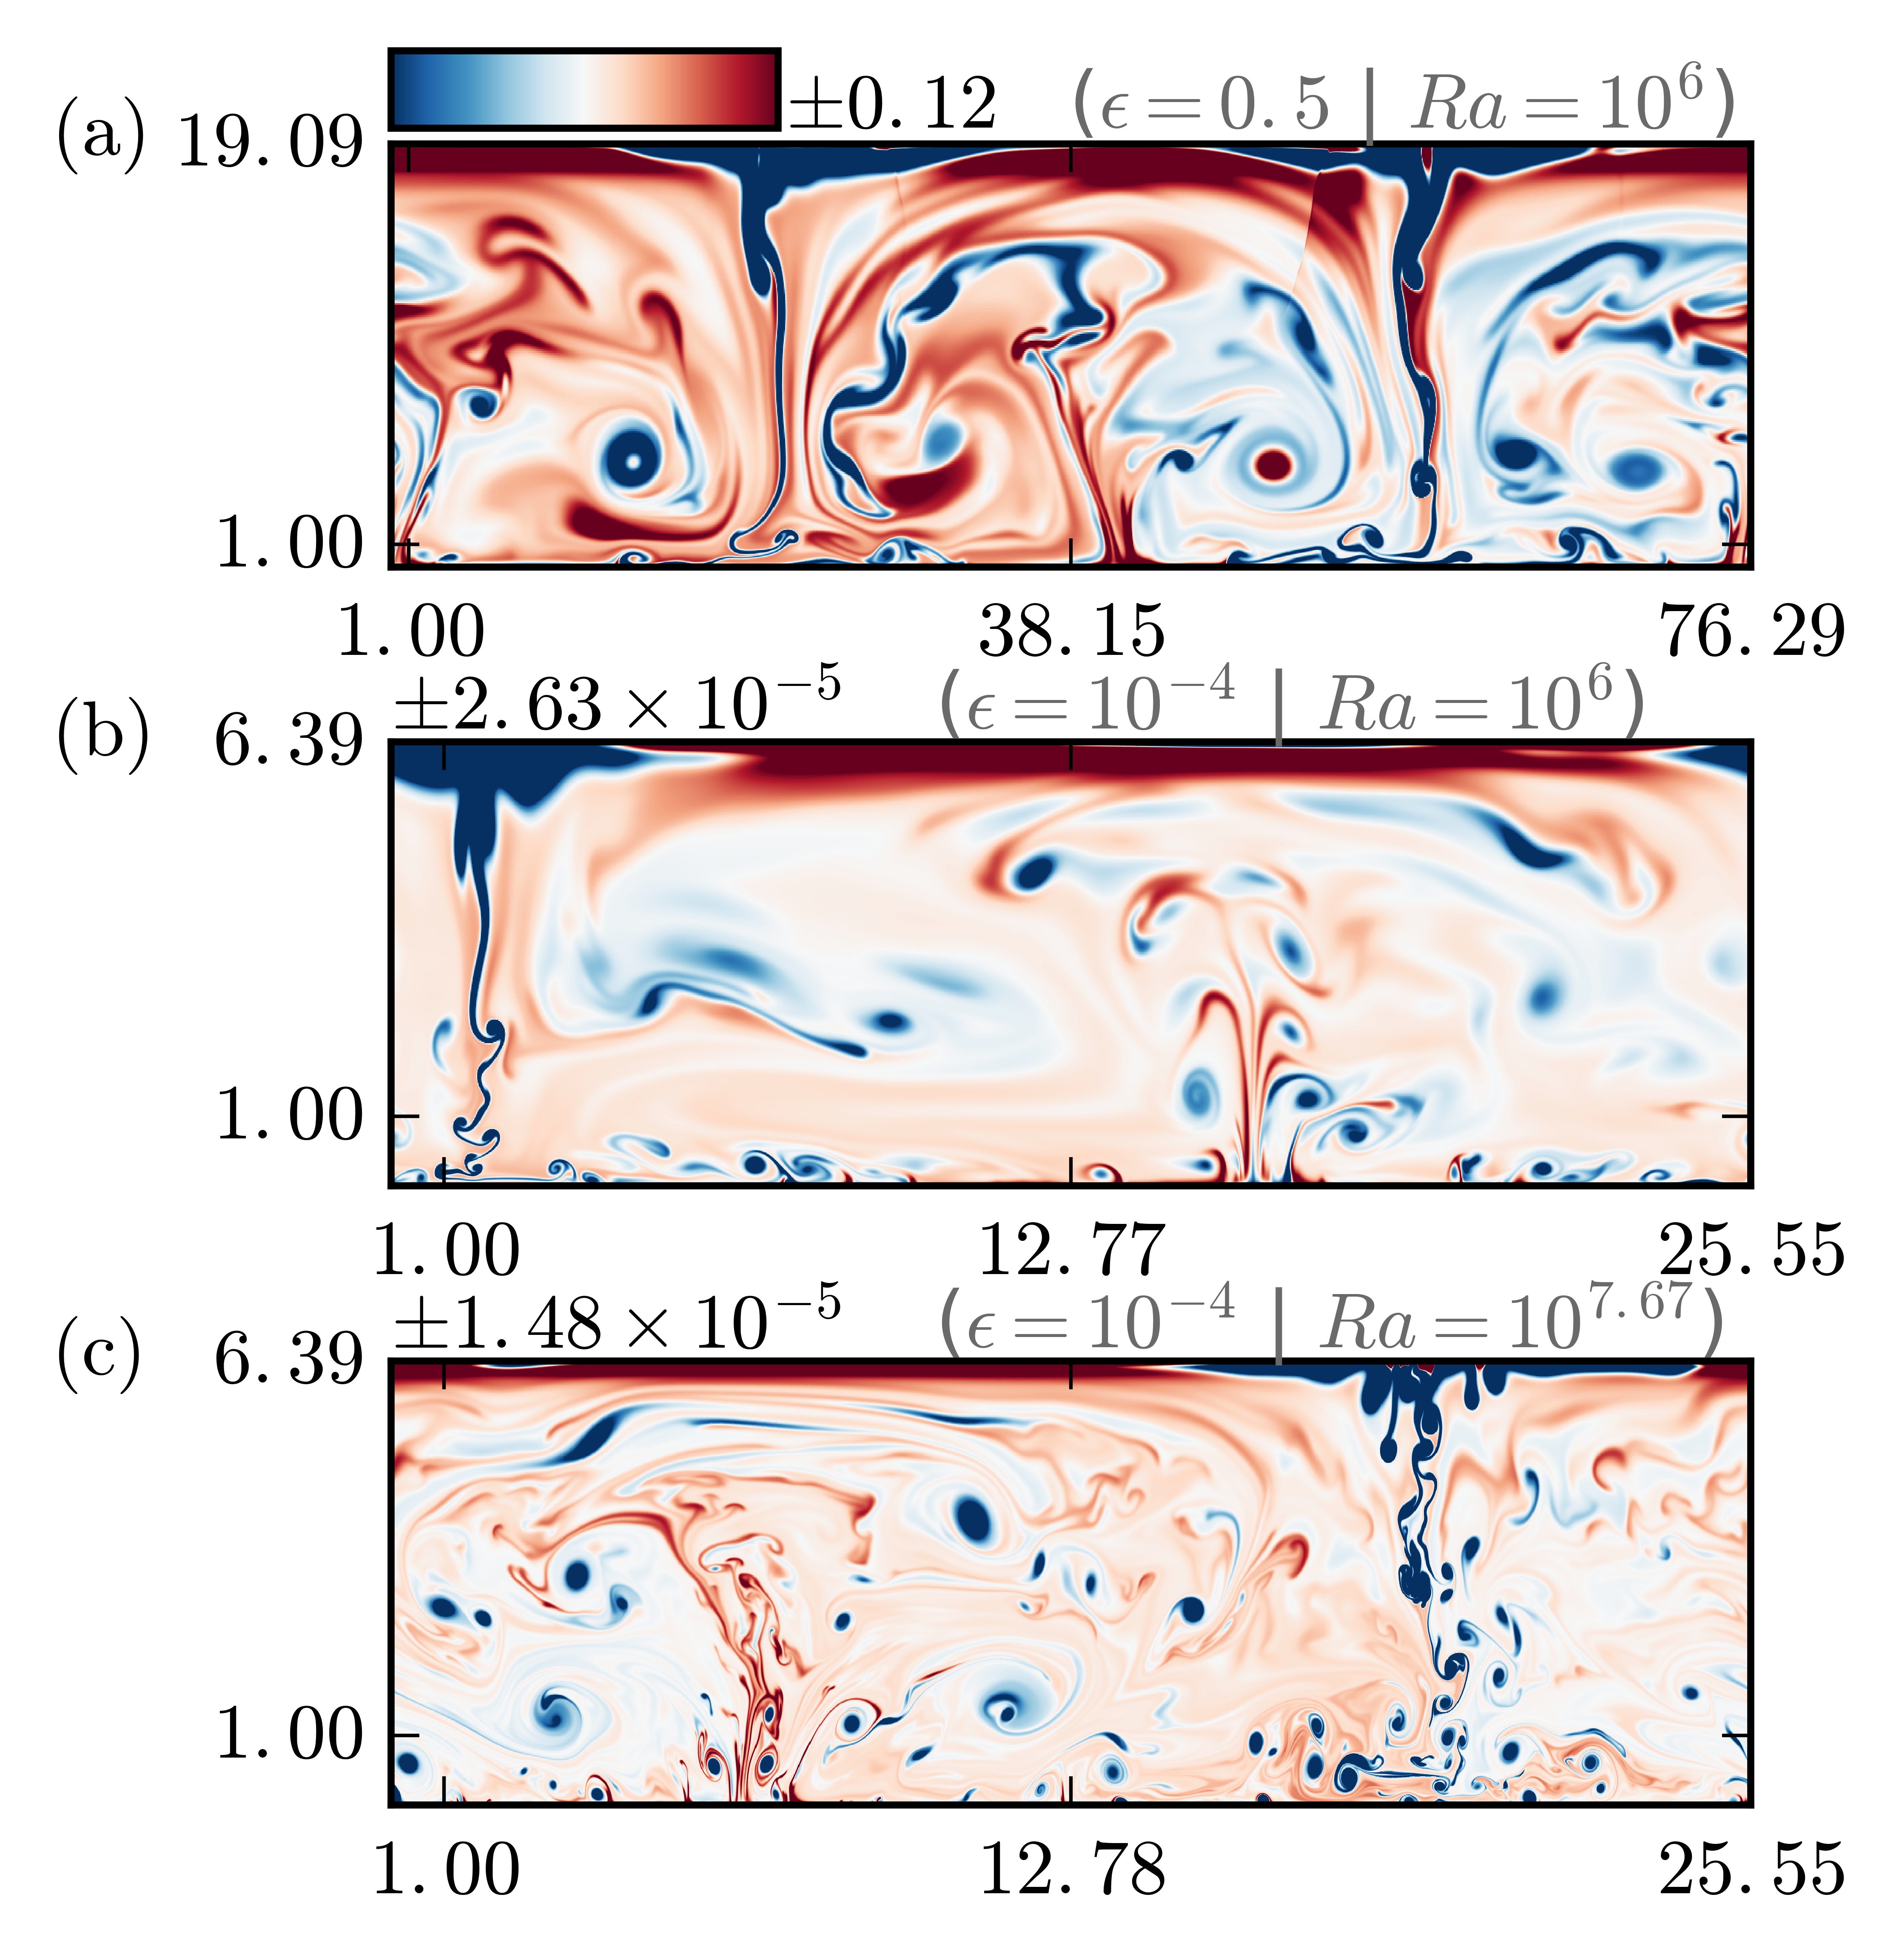
\includegraphics[width=3.4375in]{./figs/snapshots_fig.png}
\caption{Characteristic entropy fluctuations in evolved flows. 
The time- and horizontally-averaged profile is removed in all cases.  (a) At high
$\epsilon$, shock systems form near the upper downflow lanes ($x \approx 45, z \approx 15-19$)
at sufficiently high Ra.
Shock-heated fluid then flows into the downflows as the shocks propagate across upflows.
(b) At low $\epsilon$ but at the same Ra, shock systems are absent, 
but otherwise the dynamics are similar.  (c) As Ra is increased, downflows no longer span
the entirety of the domain and individual small eddies are responsible for carrying the flux.
\label{fig:entropy_snapshots} }
\end{figure}

We evolve initial value problems in which $T_1$ is
filled with infinitesimal, random white noise compared to $T_0$ and $\epsilon$.
We filter the noise spectrum in coefficient space, such that 25\% of the coefficients
have power.
Solutions were time-evolved until a long average of Nu showed little
variance with depth. By performing a linear stability analysis, 
we determined that the onset of convection
occurs at $\text{Ra}_c = \{10.06, 10.97, 10.97\}$ for $\epsilon = \{0.5, 10^{-4}, 10^{-7}\}$ respectively.  
We studied Rayleigh
numbers from values at onset up to nearly $10^6$Ra$_c$ for $\epsilon = \{0.5, 10^{-4}\}$ 
and up to $10^3$Ra$_c$ for $\epsilon = 10^{-7}$.

At large Ma ($\epsilon = 0.5$), shock systems form in the upper atmosphere near downflow lanes 
(Fig. \ref{fig:entropy_snapshots}a) once Ra is sufficiently large.
These shocks propagate through upflow regions.  
Such systems were reported in
both two \cite{cattaneo&all1990} and three \cite{malagoli&all1990} dimensional polytropic simulations previously.
These shocks heat material entering the downflows, affecting the dynamics and heat transport
of these systems.

Low Ma flows ($\epsilon = 10^{-4}$)
have similar bulk thermodynamic structures (Fig. \ref{fig:entropy_snapshots}b)
to high Ma flows.
As Ra is increased to large values 
(Fig. \ref{fig:entropy_snapshots}c), thermodynamic structures 
no longer span the whole domain but rather break up into 
small eddies which traverse the domain multiple
times before diffusing.  
While it has been suggested that pressure forces 
cause symmetry breaking in up- and downflows
\cite{hurlburt&all1984}, at low $\epsilon$ this 
effect seems to be secondary to flows obeying mass conservation as they traverse
the stratified medium.  

\begin{figure}[t]
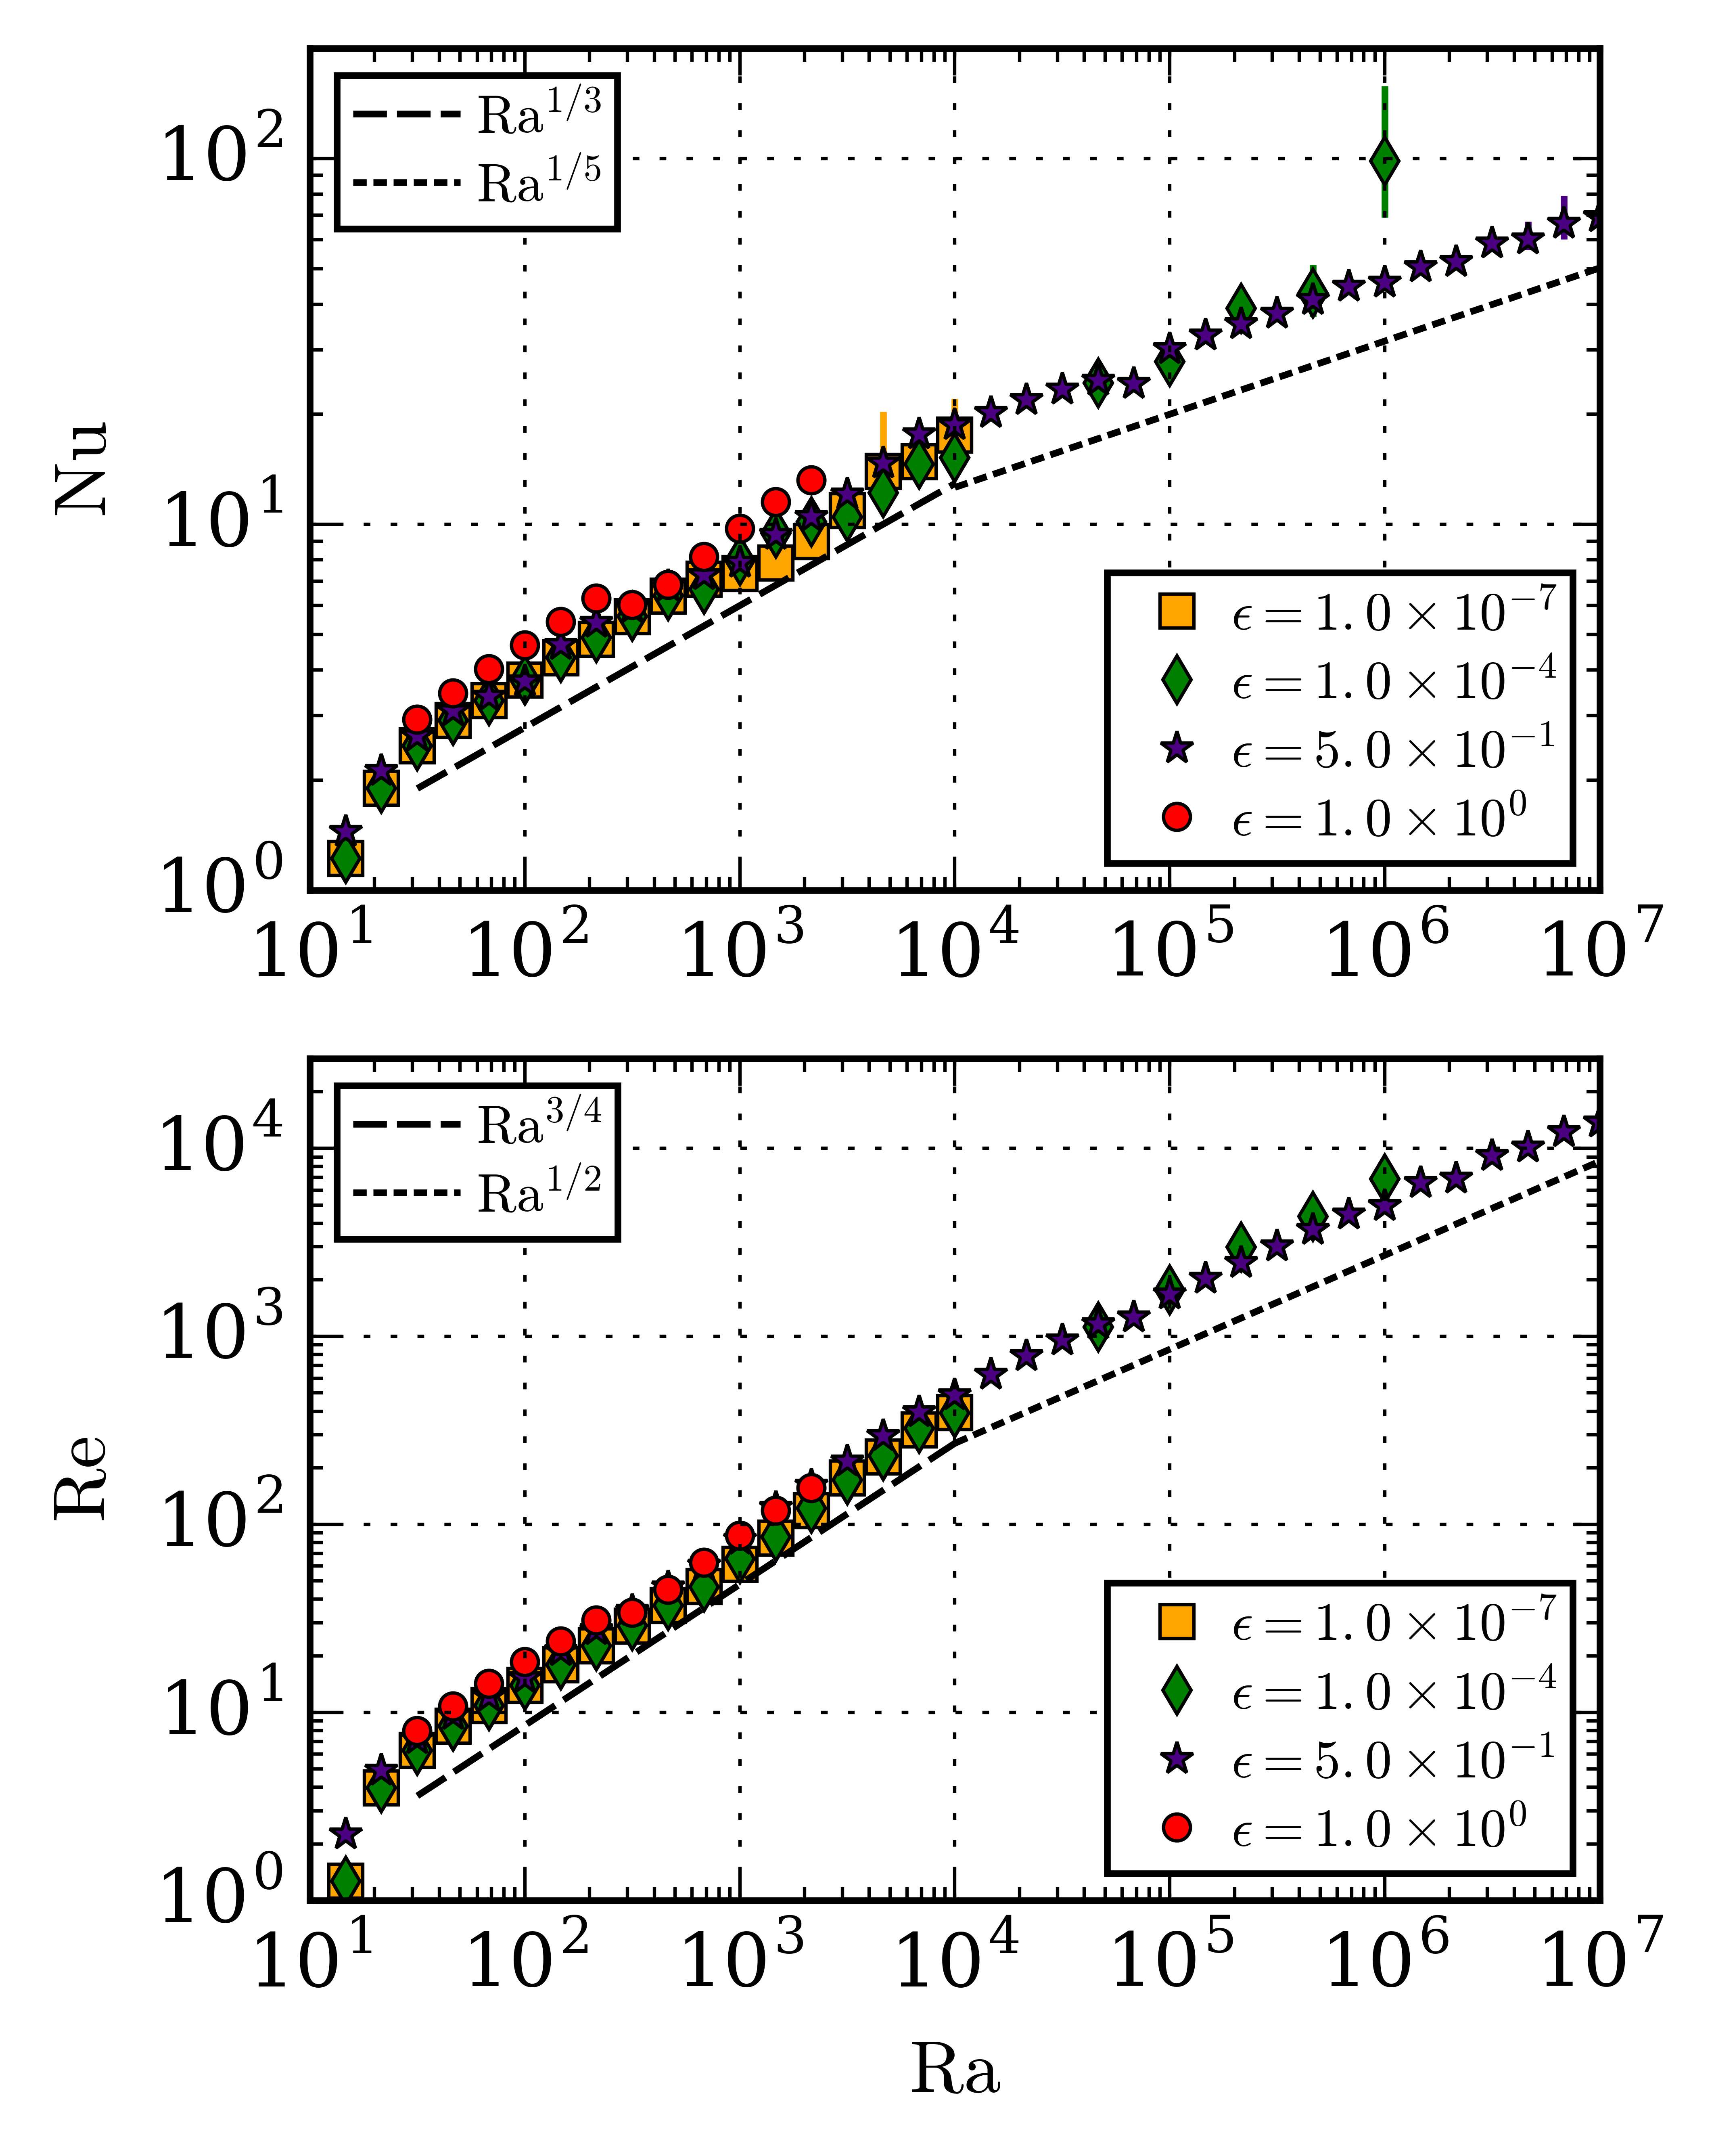
\includegraphics[width=3.4375in]{./figs/re_and_nu_v_Ra.png}
\caption{Time-averaged vertical flux profiles ($F_{\text{z}}$)
for (a) high and (b) low Ma flows at $\text{Ra }= 10^6$.  
All fluxes are defined as in (\ref{eqn:energy_eqn_full}) and 
normalized by $F_{\text{ref}} - F_{\text{A}}$, as in (\ref{eqn:nusselt}).
The dashed lines correspond to the
enthalpy flux (orange, positive) and kinetic energy flux (purple, negative).  
The grey dash-dot line is the
viscous flux and the green dotted line is the conductive flux with the 
adiabatic contribution removed. The potential energy flux is negligible and is not shown.
In (a), the viscous flux is negligible and is not shown.  The solid black line is
Nu, the properly normalized sum of all the fluxes \label{fig:re_and_nu_v_Ra} }
\end{figure}

At large enough values of Ra for shocks to form,
high Ma flows exhibit two 
local maxima in the enthalpy flux and kinetic energy flux (Fig. \ref{fig:flux_profiles}a).
Shock-heated fluid parcels sometimes gain vorticity as
they sink into the lower atmosphere.
This creates deep, rapidly-rotating regions
of mixing which persist for many overturn times. These ``spinners'' appear to
influence the dynamics, but their contributions are unclear.

At low Ma, only the deep maximum in enthalpy and kinetic energy fluxes
is present (Fig. \ref{fig:flux_profiles}b).  
Our choice of fixed-temperature boundary conditions allows the flux at the 
boundaries to vary, so many runs at $\text{Ra }> 10^5$
and $\epsilon = 10^{-4}$ exhibit states in which the flux 
entering the system at the bottom of the atmosphere 
exceeds that which leaves at the top.  
These systems are punctuated by states of vigorous shearing, similar to those previously
reported in two-dimensional RB convection \cite{goluskin&all2014}.  
%In these shearing states, flux entering the lower atmosphere approaches $F_\text{A}$,
%allowing excess energy to escape through the upper boundary.  
During shearing states, convective transport is suppressed and Nu diminishes while
excess energy exits the system through the upper boundary.
A proper long-term average over shearing
and non-shearing states retrieves an invariant Nu profile throughout the depth
of the atmosphere. 
These shearing states will be covered in more detail in a future paper. 

After appropriately time-averaging the fluxes for $\geq 200 t_b$, 
a sensible flux average is retrieved.  Nusselt numbers for
all simulations at low and high Ma are plotted as a function of Ra in Fig. \ref{fig:nu_v_ra}.  
At $\epsilon = 0.5$, in the near-sonic
regime ($\text{Ra} \leq 10^4$), the scaling of Nu with Ra is inflated,
with $\text{Nu} \propto \text{Ra}^{0.45}$, similar to that expected in the
ultimate regime of RB convection \cite{ahlers&all2009}.  As simulations
pass into the supersonic regime and shocks start to form near the downflows,
that scaling drops to $\text{Nu} \propto \text{Ra}^{0.19}$.  
At $\epsilon = \{10^{-4}, 10^{-7}\}$,
scaling laws of $\text{Nu} \propto \text{Ra}^{\{0.31, 0.31\}}$ are retrieved. 
This scaling is indistinguishable from the $\text{Ra}^{2/7}$ found in RB
convection.


\begin{figure}[t]
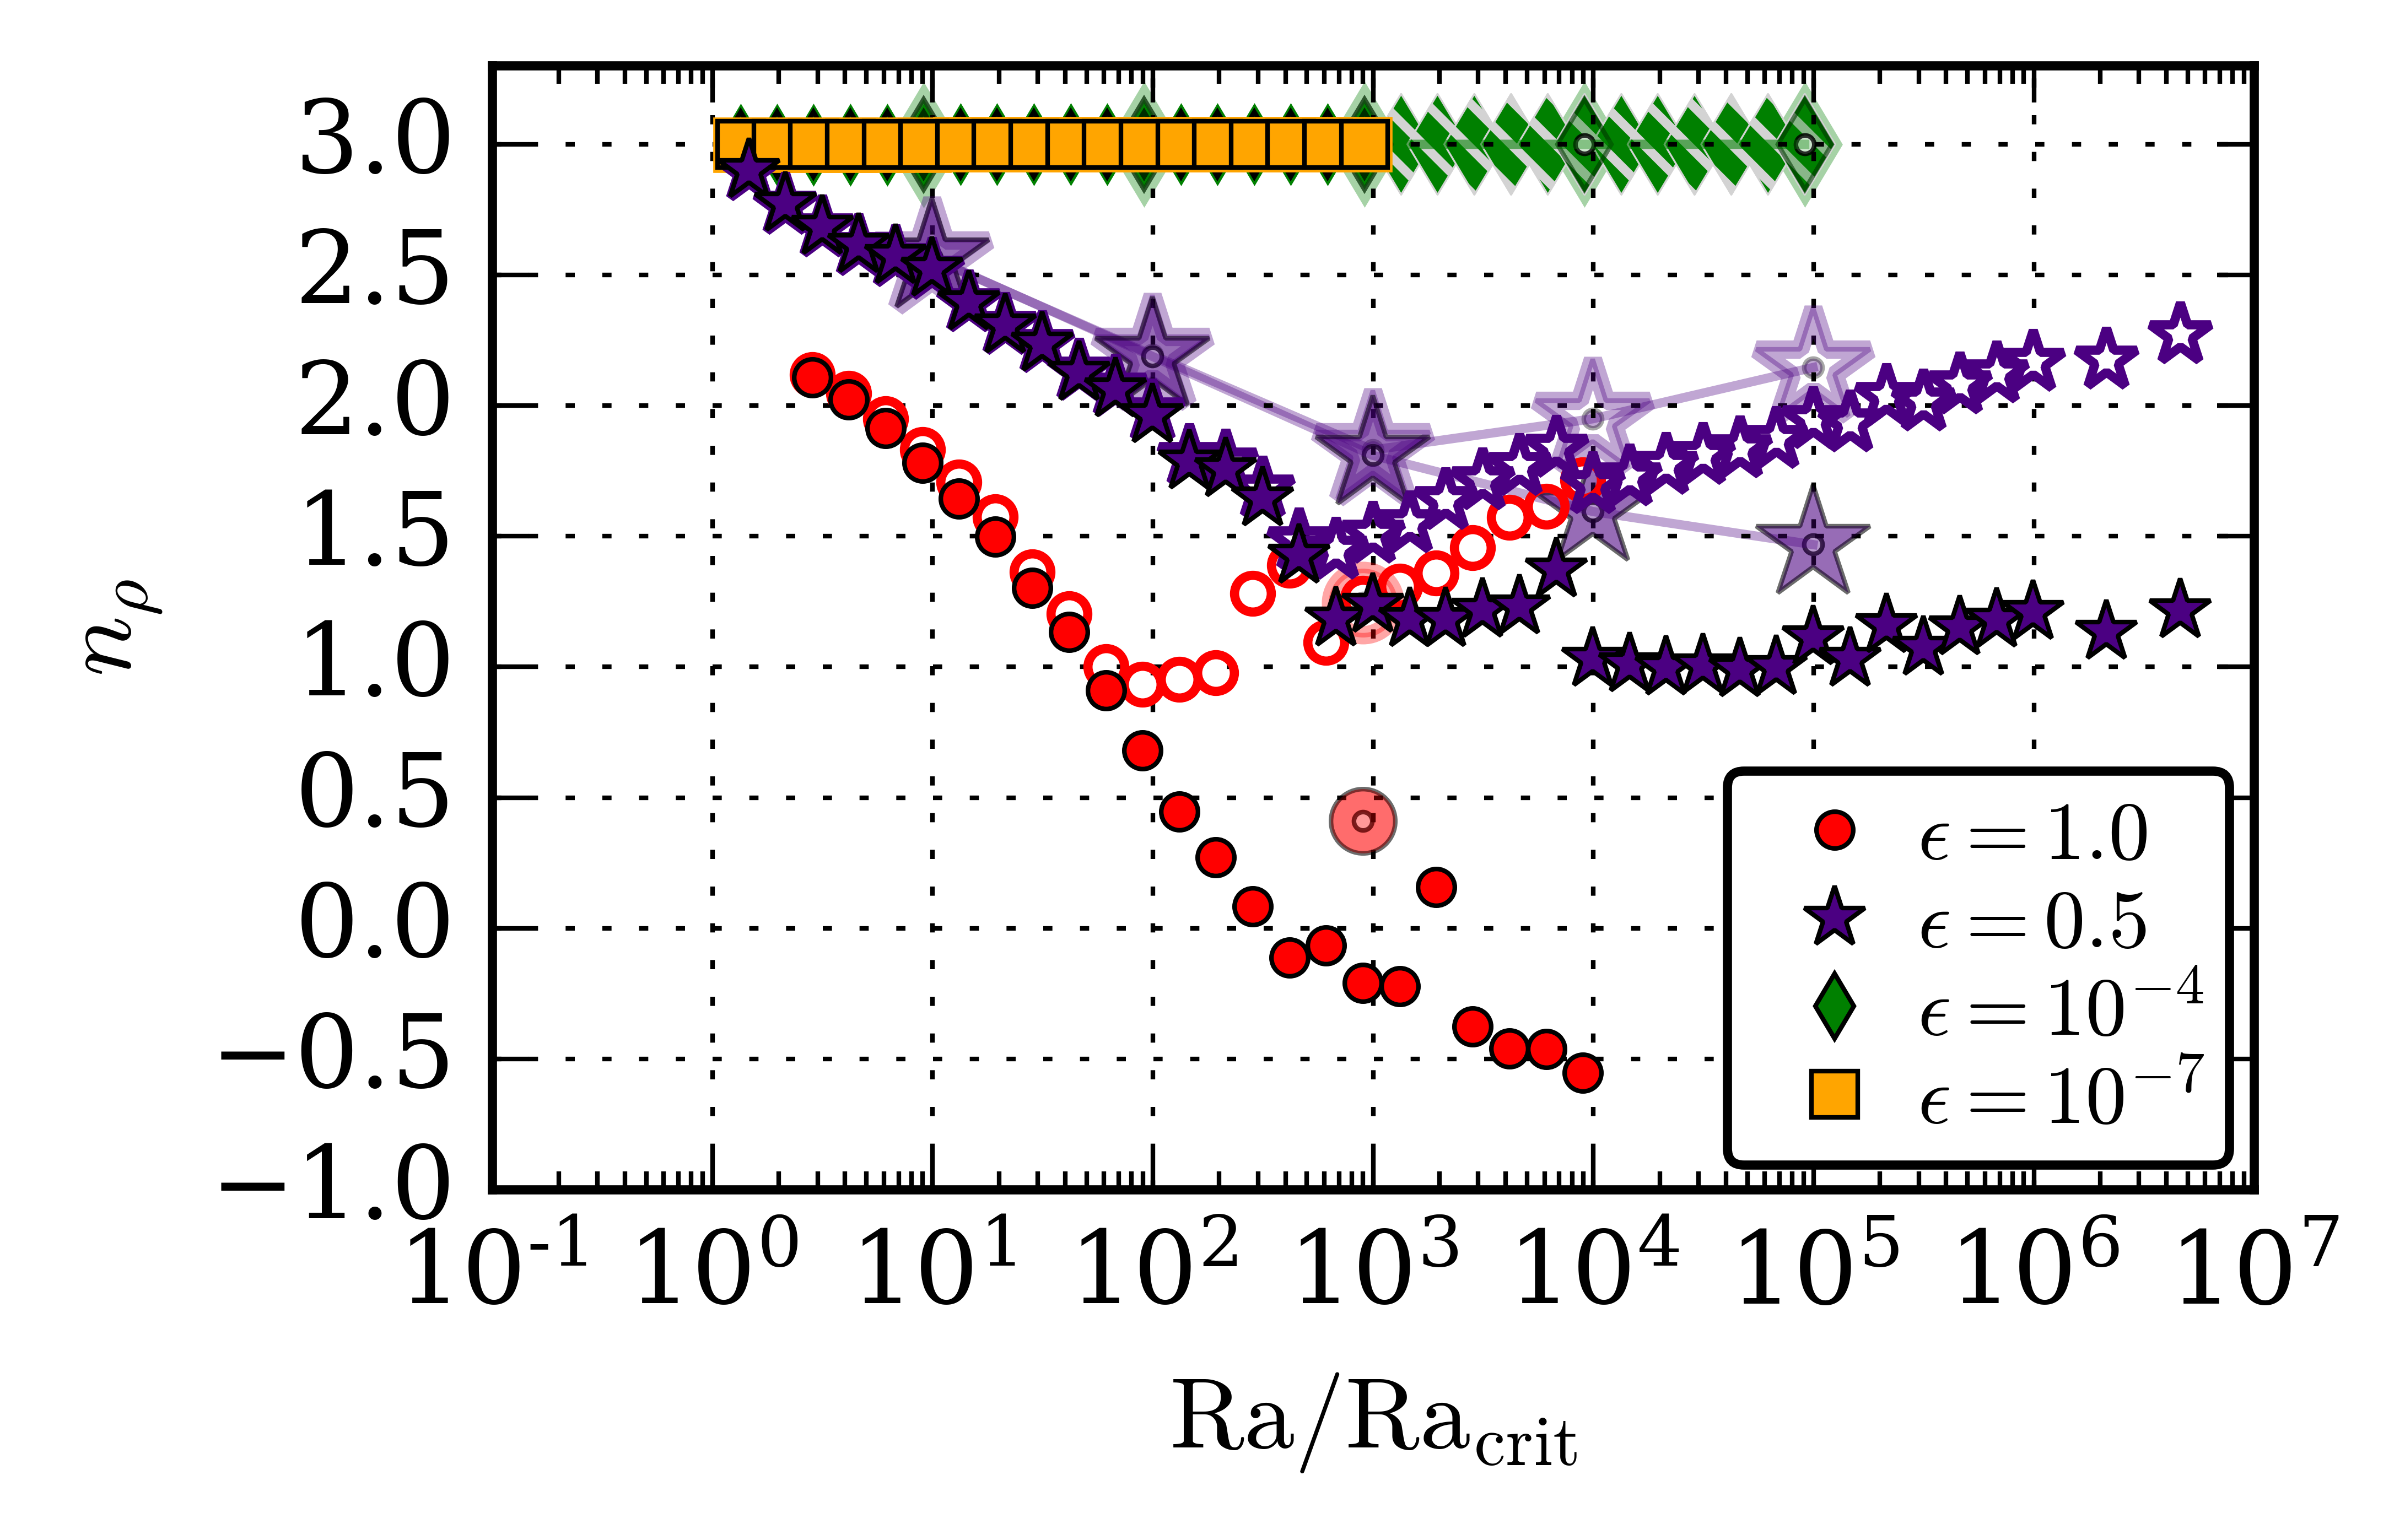
\includegraphics[width=3.4375in]{./figs/density_v_ra.png}
\caption{Variation of Nu as Ra increases at high and low $\epsilon$. 
At high $\epsilon$ (purple circles), 
a clear transition from the subsonic to supersonic regime is evident in the scaling
of Nu with Ra at $\text{Ra} \approx 10^4$.  In the low $\epsilon$ regime (green diamonds and yellow squares), 
our observed Nu scalings collapse onto a similar line which is
indistinguishable from a $\text{Ra}^{2/7}$ scaling, 
as observed in RB convection \cite{johnston&doering2009}.  Error bars are determined
 by the square root of the variance of the time-averaged Nu profile with depth and 
 indicate whether or not a solution is well-converged.
\label{fig:nrho_v_ra} }
\end{figure}

\section{Discussion}
\refstepcounter{section}
\label{sec:discussion}
In this letter we have studied fundamental heat transport by 
stratified convection in simplified 2-D polytropic
atmospheres which are specified by two additional parameters, $\nrho$ 
and $\epsilon$.  We argue that these atmospheres are the natural extension
of the RB problem to stratified systems, 
and are an ideal laboratory for understanding the basic properties of stratified
convection.  The similarity between the scaling of Nu in RB 
convection and in our low-$\epsilon$ polytropes suggests 
that a boundary layer theory such as the Grossmann-Lohse theory for incompressible flows
could be developed for fully compressible 
convection in these stratified systems \cite{ahlers&all2009}.  

The dynamics of these polytropic solutions are complex and time-dependent, even in two dimensions.
Time-dependent oscillating shear states have developed spontaneously, as seen before in RB convection
\cite{goluskin&all2014}.  While computationally difficult, the highest values of Ra and the lowest value
of $\epsilon$ studied here are far from values found in nature.  If the scalings of Nu and Ma
presented here (Figs. \ref{fig:ma_v_eps} \& \ref{fig:nu_v_ra}) hold, then under solar conditions ($\text{Ra }\approx 10^{20}$, $\text{Ma }\approx 10^{-4}$), we expect that $\epsilon \approx 10^{-20}$ and
$\text{Nu }\approx 10^{6}$.  
Solar conditions are of course more complicated, as there $\kappa$ is
set by the radiative opacity, which depends on both $\rho$ and $T$.

Future work will aim to better understand the mechanisms of shearing states and
whether or not these states are attainable in three-dimensional, non-rotating atmospheres.  Our studies
here will serve as a foundation both for understanding and comparing heat transport in stratified convection
to that in RB convection \cite{johnston&doering2009}, and for future studies of transport in stratified
convection in more realistic systems, such as rapidly rotating atmospheres \cite{julien&all2012},
atmospheres bounded by stable regions \cite{hurlburt&all1986}, 
or regions with realistic profiles of $\kappa$.



\subsection{acknowledgements}
EHA acknowledges the support of the University of Colorado's George 
Ellery Hale Graduate Student Fellowship.
This work was additionally supported by  NASA LWS grant number NNX16AC92G.  
Computations were conducted 
with support by the NASA High End Computing (HEC) Program through the NASA 
Advanced Supercomputing (NAS) Division at Ames Research Center on Pleiades
with allocations GID s1647 and GID g26133 (\textbf{AND ALSO THE NEW ONE AS OF 2017}).
We thank Axel Brandenburg, Keith Julien, Mark Rast, and Jeff Oishi for many useful discussions.

\bibliography{../biblio.bib}
\end{document}
